\section{Messung}

\subsection{Erste Messung}

\begin{frame}
	\frametitle{Erste Messungen}
	\begin{block}{Parameter}
	$U_{qpp} = 2V$, $U_B = 20V$
	\end{block}

	\begin{block}{Ausgangsignal}
	$U_{a_{pp}} = 8.1V$, $U_{RE_{pp}} = 1.85V$, $U_{R_{2_{pp}}} = 1.92V$,
	$A_V = 12.15dB$
	\end{block}

	\begin{alertblock}{Kosnequenz}
	Ein grösserer Basisstrom ist nötig $\rightarrow R_1$ kleiner oder 
	$R_2$ grösser wählen.
	\end{alertblock}	
	
\end{frame}

\begin{frame}
	\begin{figure}
		\centering
		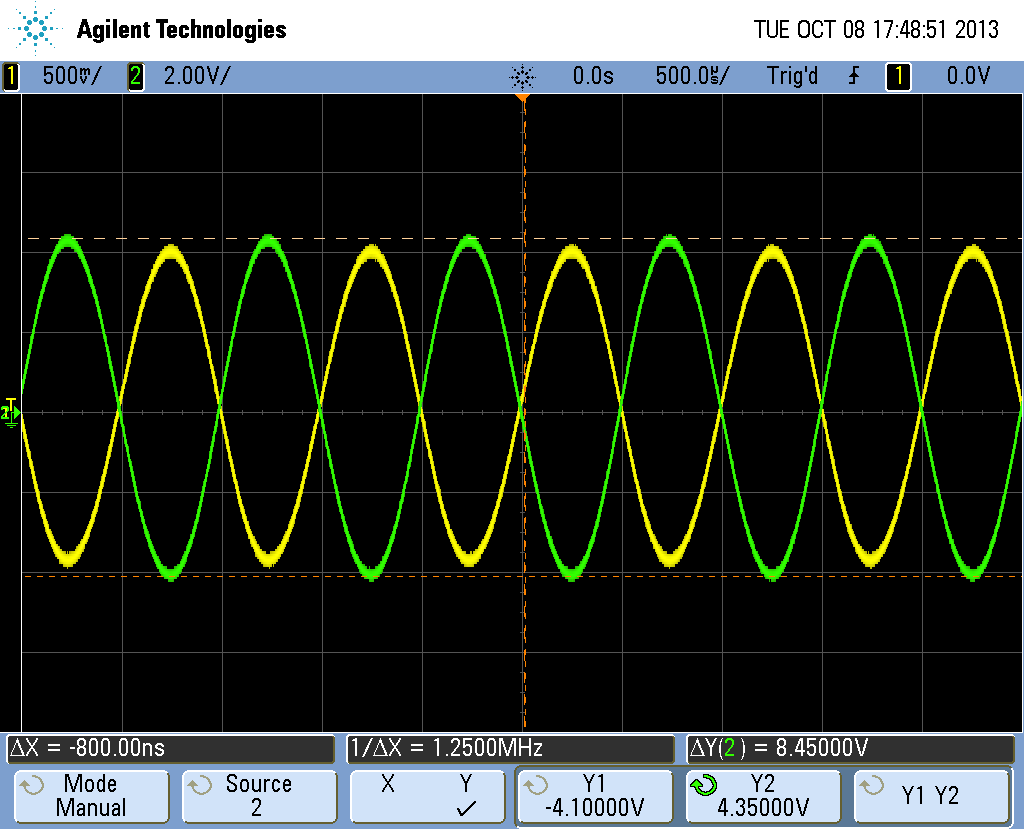
\includegraphics[width=0.7\textwidth]{scope_0.png}
		\caption{$U_a$ vs. $U_e$}
	\end{figure}
\end{frame}

\begin{frame}
	\begin{figure}
		\centering
		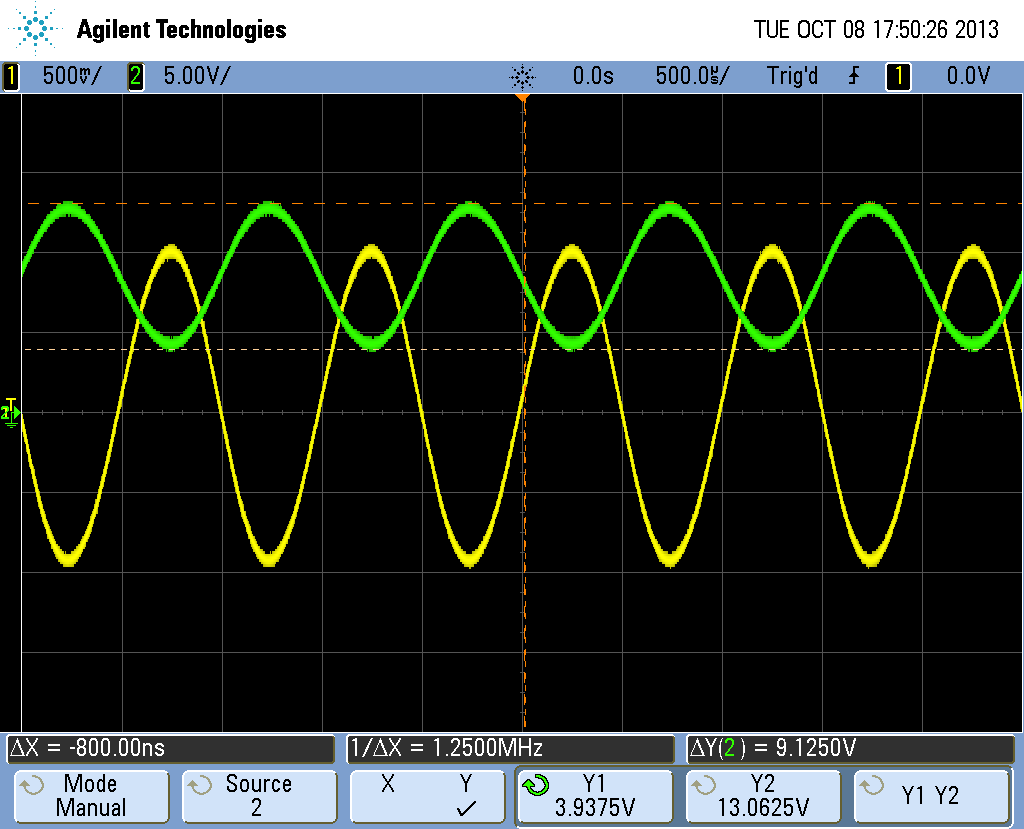
\includegraphics[width=0.7\textwidth]{scope_1.png}
		\caption{$U_C$ vs. $U_e$}
	\end{figure}
\end{frame}

\begin{frame}
	\begin{figure}
		\centering
		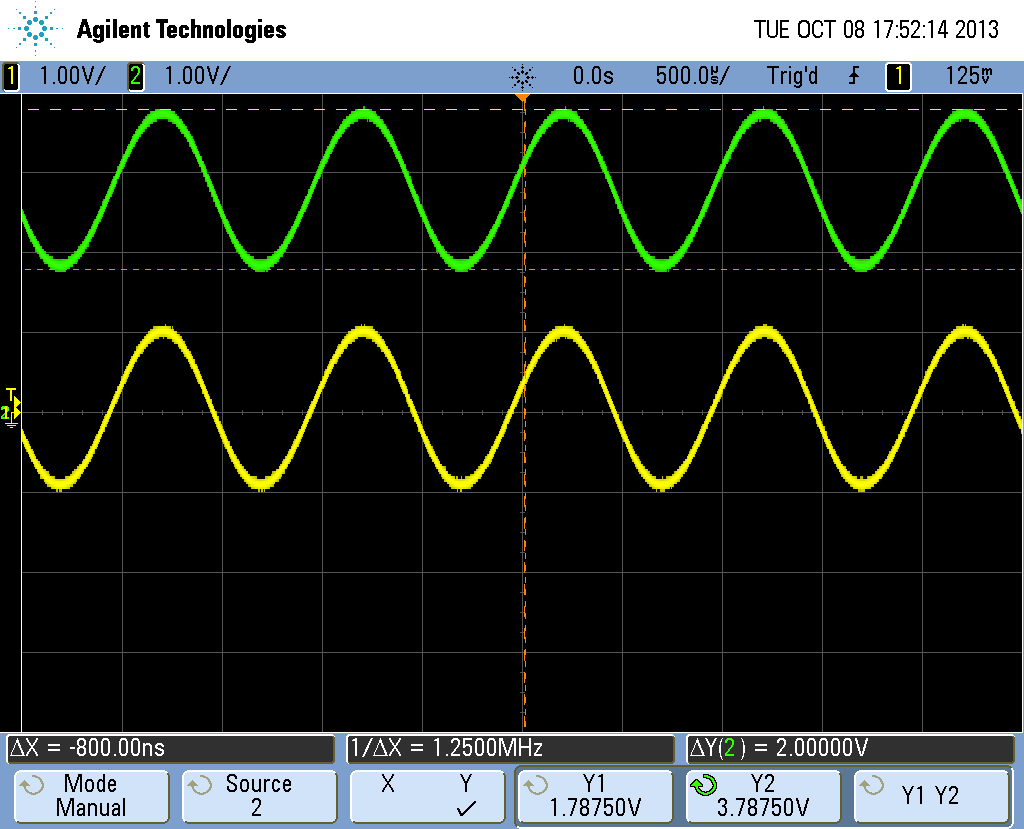
\includegraphics[width=0.7\textwidth]{scope_2.png}
		\caption{$U_{R_2}$ vs. $U_e$}
	\end{figure}
\end{frame}

\begin{frame}
	\begin{figure}
		\centering
		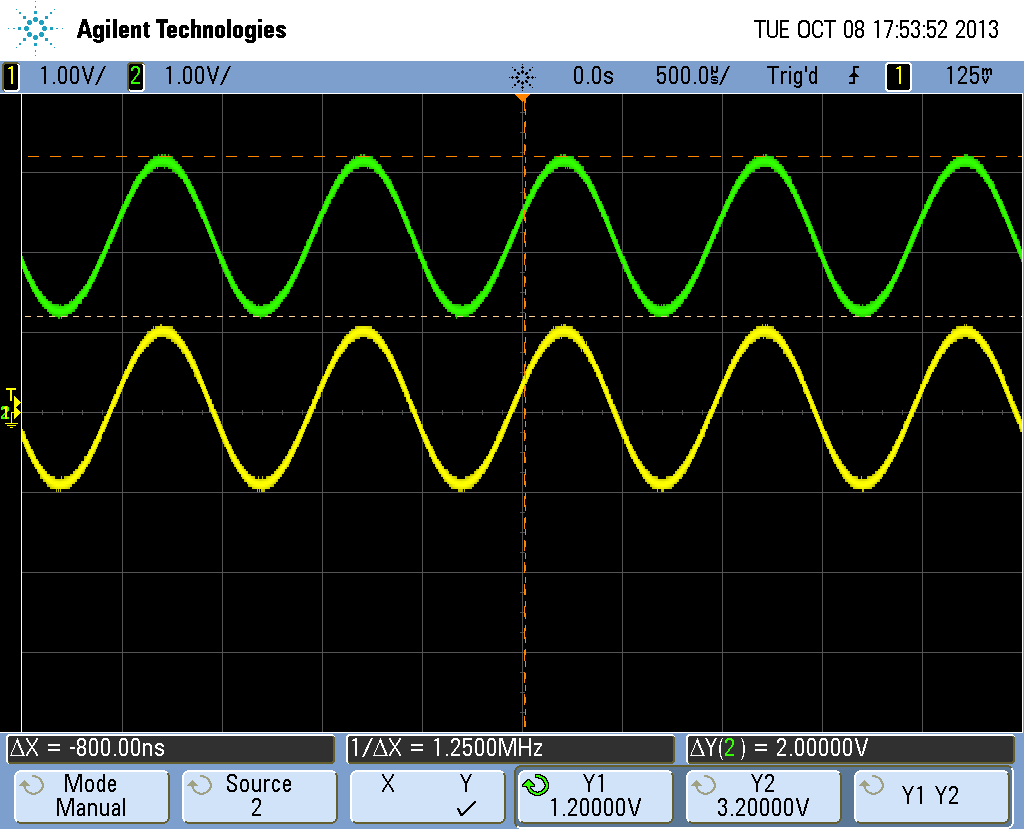
\includegraphics[width=0.7\textwidth]{scope_3.png}
		\caption{$U_{R_E}$ vs. $U_E$}
	\end{figure}
\end{frame}

\begin{frame}
	\frametitle{Anpassungen}
	\begin{enumerate}
		\item Verstärkung zu klein $\Rightarrow R_1$ verkleinern 
		\item Aussteuerungsgrenze erreicht $\Rightarrow R_2$ vergrössern
		\item Arbeitspunkt zu tief $\Rightarrow R_C$ verkleinern
	\end{enumerate}
	Mit diesen Anpassungen haben wir folgende Werte erreicht:
	\begin{itemize}
		\item $U_{q_{pp_{max}}} = 0.8V$
		\item $U_A = 3V$
		\item $A_V = 11.48dB$
	\end{itemize}
	Um den optimalen AC-Verstärker zu erstelen, müssten alle Widerstände
	aufeinander angepasst werden.
\end{frame}
